\documentclass{article}
\usepackage[margin=1in]{geometry}

\usepackage{graphicx}
\usepackage{wrapfig}
\graphicspath{img/}

\usepackage{float}


\title{Well-behaved Objects (Unit Test and Debugging) \\
        Kapitel 9}
\author{Joakim Iversen}
\date{\today}

\begin{document}
\maketitle
\newpage

\textbf{\Large Disposition:}
\begin{enumerate}
    \item Motivation
    \item Testing 
    \item Test automationer
    \item Debugging
\end{enumerate}
\newpage

\section*{Noter:}
\begin{center}
    \textit{KODE EKSEMPEL: ONLINE-SHOP}
\end{center}
\subsection*{Motivation}
I takt med at man bliver mere og mere sikker på sine evner til at skrive syntaksis korrekt kode, opstår der typisk et mere problemitisk problem forstået i logiske fejl. Disse fejl er meget sværer at opsporer, da kompileren og adnre hjælpemidle ofte ikke kan spotte dem - i det programmet egentligt ikke er i stykker, men bare ikke gør det man gerne ville have det til at gøre.

Jeg vil derfor komme ind på forskellige værktøjer vi kan gøre brug af til, at finde disse logiske fejl for at undgå bugs i vores kode.


\subsection*{Main Concepts}
\begin{itemize}
    \item Testing
    \item Unit Testing
    \item Debugging
    \item Test Automation
\end{itemize}

\subsection*{Testing og Debugging}
Det at teste et programs kode er en vigtig del af det at programmere programmer, da man ofte skal tjekke ens egne og andres programmer for fejl. Vi finder også ud af at det med at teste programmer for logiske fejl, ofte hænger sammen med det at kunne forstå andres koder, og de samme værktøjer der bruges til det ene, også viser sig brugbarer i kontekst af den anden.

\subsection*{Unit testing}
\textit{Unit Testing} refferere til det at teste enkelte dele af sit program, i modsætning til applikation testing, hvor man tester programmet i sin helhed.

\noindent - Vær dog opmæksom på at unit testing ikke reffere til en størrelse, så det vil kunne være alt fra en enkelt metode til flrer klasser og deres sammenspil i mellem -

Det er aldrig for tidligt at starter med at lave test. Og det kan faktisk nogle gange betale sig at starte på at lave test så tidligt som muligt. På den her måde vokser programmet omkring alle ens test og det er muligt at fange fejl meget tidligere end hvis man lavede programmet først. Det er også muligt løbende at se, om man er kommet til at introducere fejl til tidligere implementerede metoder i sit program.  

\subsection*{Inspector}
BlueJ har en inkoporeret inspector der tillader os at se forskellige værdier og tilstande gemt i de object vi har genereret. Den vil jeg lige tegne ud fra et \textbf{salesItem} object fra kode eksemplet \textbf{Online-Shop}:
\begin{figure}[h]
    \centering
    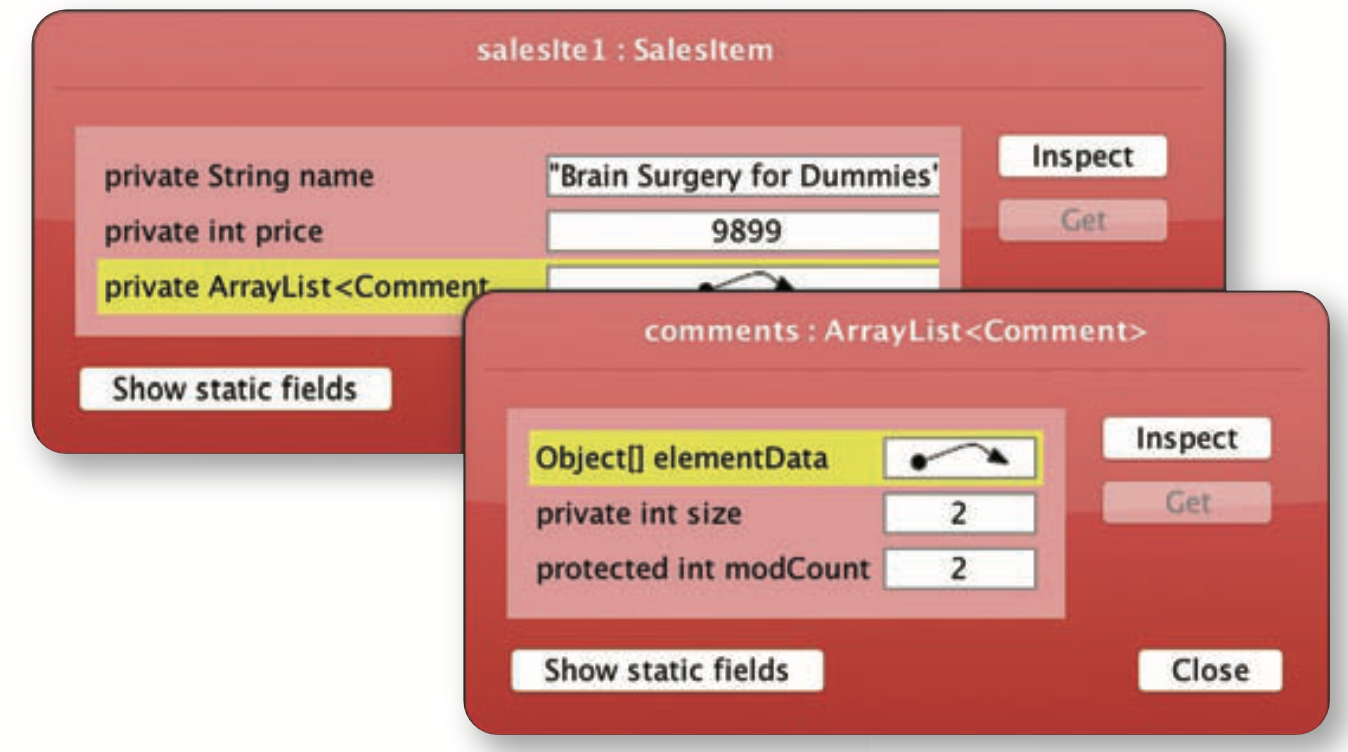
\includegraphics[scale=.2]{img/BlueJ Inspector.png}
    \caption{Tegn Figuren}
\end{figure}

Ved inspektoren kan vi følge med i hvordan de forskellige parametre udvikler sig og ændre sig i takt med at vi interagere med objektet. Her vil vi fx kunne se hvordan vores ArrayList vokser og ændre sig i takt med at vi tilføjer flere kommentarer til vores \textit{salesItem}.

En nøgle egenskab ved en god test er at man huske og teste ydergrænserne, da det ofte er her hvor der vil opstå problemer i et program.

\subsection*{Automated Test}
En af ulemperne ved at skulle teste en masse er at det ofte tager lang tid, og er kedeligt at gøre manuelt. Dette er måske ikke et problem hvis det kun skal gøre en enkelt gang, men hvis du skal teste flere hundrede gange bliver det lidt mere pro lematisk. Her kan vi derfor snakke om at gøre brug af en mere autamtiserede måde at lave test på, \textit{Regression Test}.

Regression test handler om at kører test, efter at have lavet ændringer til programmet, som tidligere er blevet godkendt.

Regression Test er implementeret i BlueJ - og flere andre Development Environments - ved brug af JUnit. JUnit er et testing framework lavet til Java sproget, og har medført en bølge af flere lignede frameworks til andre sprog. DNår vi laver en \textit{Test klasse} til en af vores java klasser opstår den lidt anderledes i blueJ. Den fremstår som en grøn firkant med teksten \textbf{\textless \textless Unit Test\textgreater \textgreater} bagved den tilsvarende klasse.

Det har også en anden funktion, hvis vi højre klikker på vores test klasse får vi nu mulugheden for at kører diverse \textit{test cases} på vores klasse i stedet for at oprette et objekt og de andre funktioner vi havde før.

Når du kører testene popper et vindue op der giver flueben ud for de test som er gået igennem, og et kryds for de test som ikke er blevet godkendt. 

Testene man kører her, vil kunne checke om følgende ting er hvad man regner med at de skal være på det givet tidspunkt. En af metoderne til JUnit er fx.
\begin{verbatim}
assertEquals(testCase, input);
\end{verbatim}

Dette vil checke om inputet er det samme som testCase og give et flueben hvis det er.


\subsection*{Andre metoder:}
\begin{itemize}
    \item Manuel gennemgang
    \begin{itemize}
        \item Gå igennem skridt for skridt med alle de forskellige funktioner der skal være tinlgængelige.
    \end{itemize}
    \item Print Statements
    \begin{itemize}
        \item Indsæt ydderlige print statements til at forstå hvordan ting ændre sig undervejs en gennemkørsel
        \item Hvilke metoder bliver kaldt
        \item Værdi af parametre
        \item Rækkefølgen metoder bliver kaldt
        \item lokale variablers værdier.
    \end{itemize}
\end{itemize}

\subsection*{Debuggers}
\begin{figure}[H]
    \centering
    \textit{TEGN DEBUGGEREN:} \\
    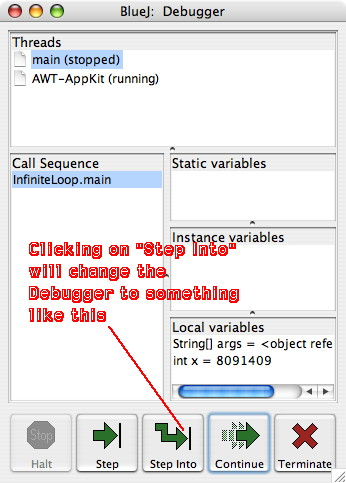
\includegraphics[scale=0.4]{img/loopInfin_debuggerStepInto.jpg}
\end{figure}

Forklar hvordan debuggeren virker undergennemkørsel.

\subsection*{Hvilken metode skal bruges}
Skrevne og verbale gennemgang er gode at gennemgå nyligt skrevet kode, forstå hvordan et program virker eller til debugging.
Fordelen ved dem er at de er nemme at bruge og virker i alle programmeringssprog. 
Ulempen er at de ikke er nemme at gentage. Derfor virker det fint til at debugge, men dårligt til at teste. 

Derfor er regression test bedre til at test, da de tillader os at ahve en masse, let gentagelige, testcases vi hurtigt kan gentage på vores program. Fordellen er også at når testene først er sat op kan vi hurtigt kører de samme test på vores program efter ændtinger, og på den måde se om det stadig virker efter hensigten.
\end{document}
